\section{La ricerca dei punti fissi di una popolazione}
Consideriamo una popolazione la cui evoluzione sia descritta dall'equazione logistica \ref{eq:logistica}, che, ricordiamo, è $$ x_{i+1} = r x_i (1-x_i)$$ La domanda più interessante che ci si può porre riguardo alla sua evoluzione è come si comporti il numero di individui normalizzato $x_i$ asintoticamente, ovvero nel limite per $i\rightarrow \infty$. In particolare, ci si chiede se esistano dei valori "di equilibrio", $x_{eq}$, tali che, una volta raggiunti, il risultato delle iterazioni successive si mantenga costante, ovvero tali che $$r x_{eq} (1-x_{eq}) = x_{eq}$$
Tali punti, se esistono, vengono chiamati \textit{punti fissi} dell'equazione logistica.

\subsection{Punti fissi di una funzione e metodo delle iterazioni}
In termini generali, data una funzione $f$,  cercarne i punti fissi significa cercare quei valori di $x$ per cui 
\begin{equation}
    x = f(x)
    \label{eq:punto_fisso}
\end{equation}
Un modo per trovare i punti fissi di una funzione è, naturalmente, quello di risolvere l'equazione \ref{eq:punto_fisso} in modo analitico, quando possibile. Dal momento che questo potrebbe però non essere sempre possibile, un altro metodo per trovare alcuni dei punti fissi di una funzione è il cosiddetto \textit{metodo delle iterazioni}: si parte da un valore $x_0$ scelto arbitrariamente e si calcola $f(x_0) =: x_1$; successivamente si prende $x_1$ e si calcola $f(x_1) =: x_2$. Si prosegue in questo modo, ottenendo una successione definita in modo iterativo:
\begin{equation}
    x_{n+1} = f(x_n)
    \label{eq:ricorsione}
\end{equation}
Se il risultato delle iterazioni tende a stabilizzarsi attorno a un valore, ovvero esiste finito il limite per $n \rightarrow \infty$ di $x_n$, tale valore rappresenta proprio un punto fisso $x_{eq}$ soddisfacente l'equazione \ref{eq:punto_fisso}. Si può intuire che tale metodo non permette di trovare tutti i punti fissi di una funzione, in primo luogo perché il valore trovato asintoticamente potrebbe dipendere dalla scelta iniziare di $x_0$, e in secondo luogo perché il metodo delle iterazioni permette di trovare solo i cosiddetti \textit{punti fissi attrattori}, vale a dire quei valori che sono il limite asintotico delle successioni appena definite. Non si raggiungono infatti i \textit{punti fissi repulsori}, che sono sempre punti soddisfacenti l'equazione \ref{eq:punto_fisso}, ma per i quali si verifica che, se si parte da un valore $x_0$ vicino ad essi, le successioni ricorsive definite in \ref{eq:ricorsione} divergono da essi per andare a convergere verso altri punti fissi (che saranno attrattori). 

Per una popolazione, si può interpretare la differenza tra punti fissi attrattori e repulsori nel modo seguente: se si immagina di perturbare il numero di individui della popolazione spostandolo da un valore di equilibrio, i punti fissi attrattori sono quelli per cui la popolazione si riporta allo stato di equilibrio iniziale, mentre i punti fissi repulsori sono quelli per i quali la popolazione si allontana dal valore di equilibrio iniziale. Si può quindi pensare ai punti fissi attrattori e repulsori come a stati di equilibrio stabili o instabili, in analogia con gli stati di equilibrio dei sistemi fisici. Questa definizione della natura dei punti fissi può essere formalizzata nel seguente modo:
\begin{definizione}{\textnormal{\textbf{Punto fisso attrattivo e punto fisso repulsivo}}}

    Sia $x_{eq}$ un punto fisso di una funzione $f$. $x_{eq}$ è detto \textnormal{punto fisso attrattivo} se, in un intorno di $x_{eq}$, $$\left|f(x_{eq} + \delta x) - f(x_{eq})\right| < \left|\delta x\right|$$
    Viceversa, $x_{eq}$ è detto punto fisso repulsivo se, in un intorno di $x_{eq}$, $$\left|f(x_{eq} + \delta x) - f(x_{eq})\right| > \left|\delta x\right|$$
    \label{def:attrattore_repulsore}
\end{definizione}

Prima di andare a ricavare un criterio per stabilire la natura di un punto fisso, può essere interessante vedere come il metodo delle iterazioni possa essere interpretato graficamente. Rappresentando la variabile $x$ sull'asse delle ascisse e la funzione $f(x)$ sull'asse delle ordinate, il metodo delle iterazioni si traduce nelle seguenti azioni: partendo da un valore iniziale $x_0$, si sale fino a incontrare il punto sul grafico di $f$ di ascissa $x_0$, vale a dire $(x_0, f(x_0)$; l'ordinata di tale punto deve ora diventare l'ascissa della successiva iterazione, quindi si può tracciare la bisettrice e, partendo dal punto trovato, muoversi orizzontalmente verso di essa, dove si incontrerà il punto $(f(x_0), f(x_0))$. Si può ora ripetere la procedura partendo da questo punto, muovendosi verticalmente fino a incontrare il punto $\left(f(x_0 ) , f(f(x_0)) = x_1 \right)$, muovendosi poi verso la bisettrice, e avanti così. Si osserverà che questo metodo permette di convergere a un punto fisso di $f$, che si troverà all'intersezione tra il grafico di $f$ e la bisettrice. Si può inoltre osservare che ci sono alcuni punti che, pur essendo intersezioni tra il grafico e la bisettrice, non sono mai il limite asintotico del metodo delle iterazioni: sono punti fissi repulsori.

Nella figura \ref{fig:iterazioni} è presente un esempio con $f(x) = x^2$. Si può osservare che i punti fissi sono $x = 0$ e $x=1$, come si ricava facilmente in modo analitico, che sono infatti i punti di intersezione tra la parabola e la bisettrice. Inoltre sono state rappresentate alcuni iterazioni partendo da valori iniziali diversi, che permettono in particolare di vedere come non importa quanto vicino a $x=1$ inizino le iterazioni, non si converge mai a $x = 1$, punto fisso repulsore.

\begin{figure}[h!]
    \begin{center}
    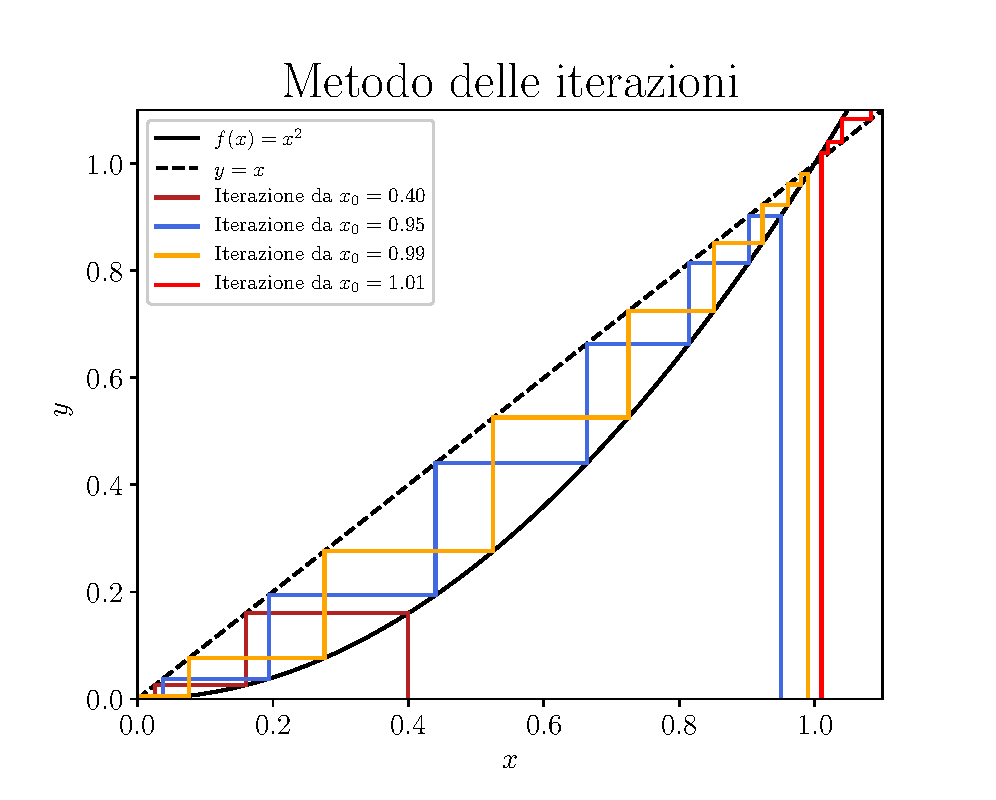
\includegraphics[scale=0.7]{Immagini/iterazioni.eps}
    \captionsetup{width=.8\linewidth}
    \caption{I punti fissi di $f(x) = x^2$ sono le intersezioni tra la funzione e la bisettrice. Il metodo delle iterazioni applicato ad $f$ mostra che le iterazioni convergono sempre a $x=0$, punto fisso attrattore, se si parte da un valore iniziale $0<x_0<1$. Se si parte invece da un valore $x_0 > 1$ le iterazioni divergono all'infinito. Il punto fisso $x=1$ invece non viene mai raggiunto, per quanto vicino vi si parta, ed è infatti repulsore.}
    \label{fig:iterazioni}
    \end{center}
\end{figure}


\subsection{Un criterio per stabilire la natura dei punti fissi}
Come è possibile, in generale, sapere se una funzione ammette punti fissi, e, nel caso in cui questi siano ricavabili per via analitica o per successioni, come è possibile stabilirne la natura? Fortunatamente, per quanto riguarda l'esistenza di punti fissi, un teorema qui non dimostrato ne assicura l'esistenza per tutte le funzioni continue definite da un insieme chiuso in se stesso. Per quanto riguarda invece la determinazione della natura dei punti fissi, il seguente teorema fornisce un criterio per stabilire la repulsività o attrattività dei punti fissi di una funzione, che in molti casi risulta di utile applicazione.

\begin{teorema}
Sia $A\subset \mathbb{R}$ chiuso, sia $f : A \rightarrow A$ una funzione derivabile in A e sia $x_{eq}$ un punto fisso per f. Allora $x_{eq}$ è un punto fisso attrattore per $f$ se e solo se 
\begin{equation}
    \left| \dfrac{\dif f(x)}{\dif x}\right| _{x_{eq}} < 1
    \label{eq:attrattore}
\end{equation}
Viceversa, $x_{eq}$ è un punto fisso repulsore per $f$ se e solo se
\begin{equation}
    \left| \dfrac{\dif f(x)}{\dif x}\right| _{x_{eq}} > 1
    \label{eq:repulsore}
\end{equation}
\label{teorema}
\end{teorema}
\begin{proof}[Dimostrazione]
    
    Dimostriamo la condizione \ref{eq:attrattore} per un attrattore, quella per un repulsore è analoga. Richiamiamo la definizione di punto fisso repulsore data nella Definizione \ref{def:attrattore_repulsore}:
    $$|f(x_{eq} + \delta x) - f(x_{eq})| < |\delta x|$$
    Dal momento che $f$ è derivabile, si può sviluppare al prim'ordine la funzione attorno a $x_{eq}$
    $$ |\delta x| \left| \dfrac{\dif f(x)}{\dif x} \right|_{x_{eq}} + o(|\delta x|) < |\delta x|$$
     dividendo per $|\delta x|$ e facendo il limite per $\delta x \rightarrow 0$ si ottiene infine
    $$ \left| \dfrac{\dif f(x)}{\dif x}\right| _{x_{eq}} < 1$$
\end{proof}